\subsection{Diagramme de Déploiement}

Les diagrammes de déploiement montrent la disposition physique des différents matériels appelés nœuds(ordinateurs, périphériques, réseaux, systèmes de stockage...) qui entrent dans la composition d’un système et la répartition des instances de composants, processus et objets qui vivent sur ces matériels. Les diagrammes de déploiement sont donc très utiles pour modéliser l’architecture physique d’un système.

\begin{minipage}{1,2\textwidth}
	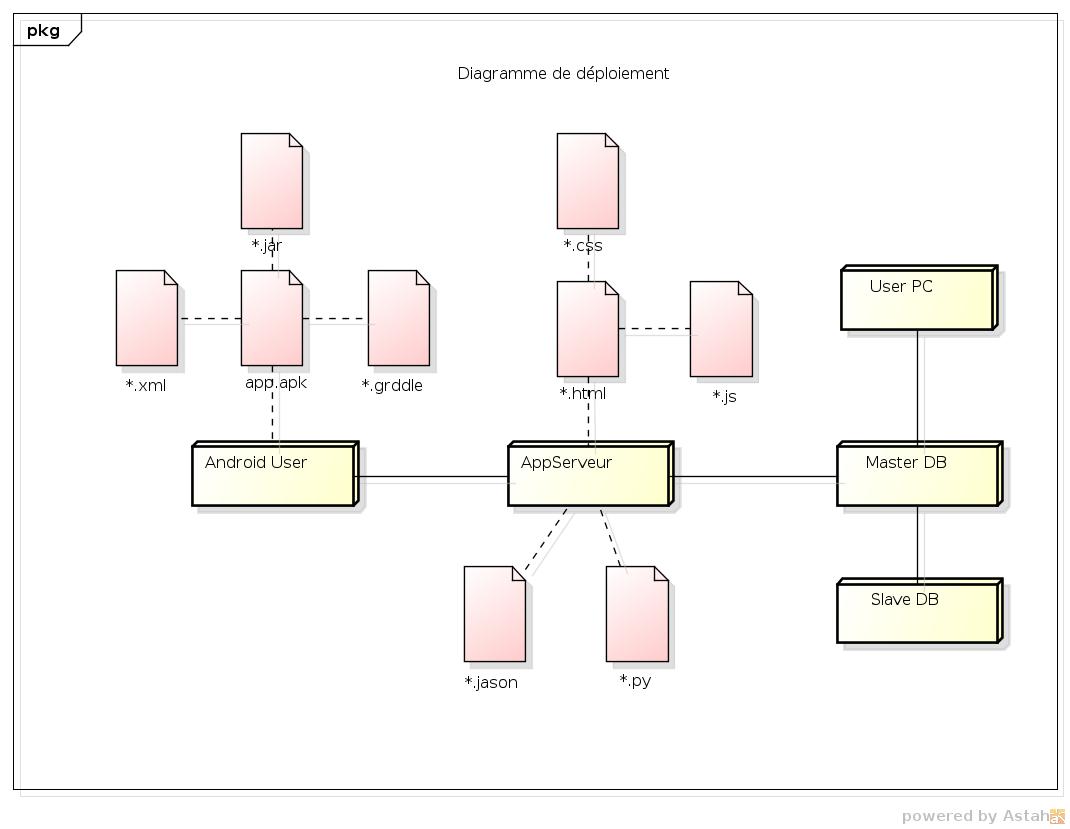
\includegraphics[width=0.7\linewidth]{mama/images/Deployment}
	\label{fig:deployment}
\end{minipage}
\hspace*{\stretch{1}}


 C'est en partant de ces diagrammes qu'on écrit le code informatique pour répondre aux besoins des utilisateurs.


